\documentclass{article}
\usepackage{amsmath,amssymb,amsthm,latexsym,paralist}
\usepackage{graphicx}
\usepackage{verbatim}

\theoremstyle{definition}
\newtheorem{problem}{Problem}
\newtheorem*{solution}{Solution}
\newtheorem*{resources}{Resources}

\newcommand{\name}[1]{\noindent\textbf{Name: #1}}
\newcommand{\honor}{\noindent On my honor, as an Aggie, I have neither
  given nor received any unauthorized aid on any portion of the
  academic work included in this assignment. Furthermore, I have
  disclosed all resources (people, books, web sites, etc.) that have
  been used to prepare this homework. \\[1ex]
 \textbf{Signature:} \underline{\hspace*{5cm}} }

%  \newcommand{\checklist}{\noindent\textbf{Checklist:}
% \begin{compactitem}[$\Box$] 
% \item Did you add your name? 
% \item Did you disclose all resources that you have used? \\
% (This includes all people, books, websites, etc. that you have consulted)
% \item Did you sign that you followed the Aggie honor code? 
% \item Did you solve all problems? 
% \item Did you submit (a) the pdf file of your homework?
% \item Did you submit (b) a hardcopy of the pdf file in class? 
% \end{compactitem}
% }



\newcommand{\problemset}[1]{\begin{center}\textbf{Problem Set
      #1}\end{center}}
\newcommand{\duedate}[2]{\begin{quote}\textbf{Due dates:} Electronic
    submission of the pdf file of this homework is due on
    \textbf{#1} on ecampus, a signed paper copy of the pdf file is due
    on \textbf{#2} at the beginning of class. \end{quote} }

\newcommand{\N}{\mathbf{N}}
\newcommand{\R}{\mathbf{R}}
\newcommand{\Z}{\mathbf{Z}}


\begin{document}
\problemset{4}
\duedate{2/21/2019 before noon}{2/21/2019}
\name{ Hunter Cleary }
\begin{resources} (All people, books, articles, web pages, etc. that
  have been consulted when producing your answers to this homework)
  \begin{itemize}
      \item https://en.wikipedia.org/wiki/Memoization
      \item Longest common subsequence algorithm -- example
      \\https://www.youtube.com/watch?v=P-mMvhfJhu8
      \item https://www.geeksforgeeks.org/longest-increasing-subsequence-dp-3/
      \item https://people.eecs.berkeley.edu/~nirkhe/cs38notes
  \end{itemize}
\end{resources}
\honor

\newpage
Make sure that you describe all solutions in your own words. Re-read
chapters 15 and 16 in our textbook. 

\begin{problem}[20 points]
Solve Exercise 15.3-2 on page 389 of our textbook. 
\end{problem}
\begin{solution} \\
\\
Merge Sort with 16 Elements
\\
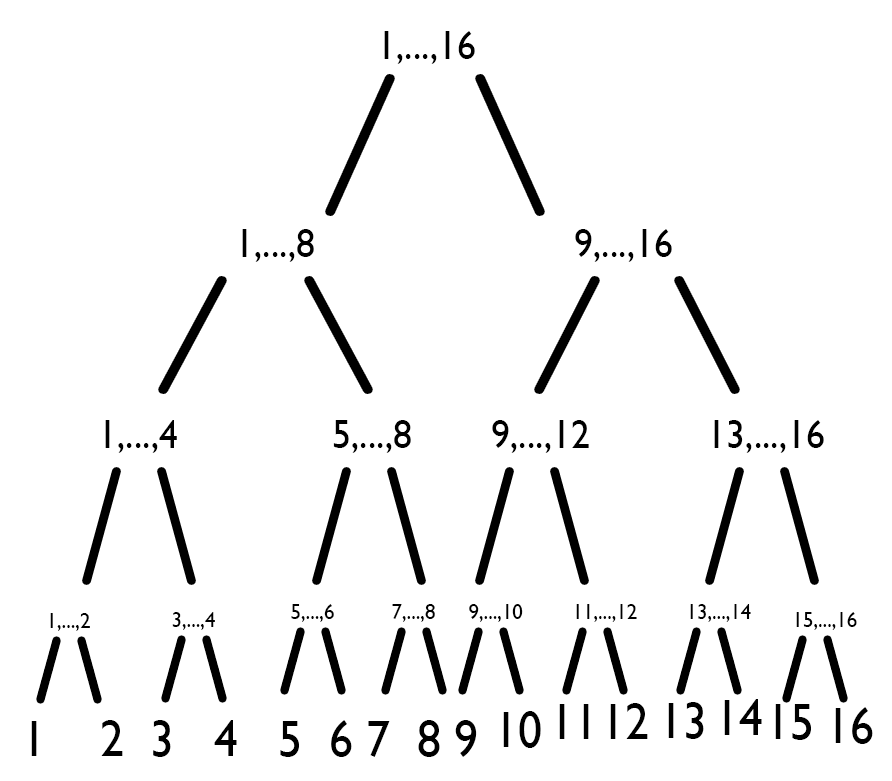
\includegraphics[width = 9cm]{recursiontree.png}
\\
Memoization is not effective because none of the comparisons are made more than once. Since none of the results are used more than once, storing them does not speed up the algorithm.
\\
\\
\end{solution}
\\
\\
\begin{problem}[20 points]
Solve Exercise 15.4-1 on page 396 of our textbook. 
\end{problem}
\begin{solution} \\
\\
Determining a Longest Common Subsequence\\
\\
$<1,0,0,1,0,1,0,1>$ and $<0,1,0,1,1,0,1,1,0>$\\
\\
The longest common subsequence is $<1,0,0,1,1,0>$\\
\\

\end{solution}

\newpage

\begin{problem}[30 points]
Solve Exercise 15.4-5 on page 397 of our textbook. 
\end{problem}
\begin{solution} \\
\\
Give an $O(n^2)$-time algorithm to find the longest monotonically (entirely) increasing subsequence of a sequnce of numbers.
\\
\begin{verbatim}
    S[]; //sequence S contains 'n' numbers
    LIS[]; //LIS is the longest increasing subsequence
    int longestLength;
    for (int i = 1 ; i < n ; i++){
        for (int j = 0 ; j < i-1 ; j++){
            if ( S[i] > S[j] && LIS[j] + 1 > LIS[i] ){
                LIS[i] = LIS[j] + 1;
            }
        }
    }
    //finding maximum length subsequence
    for(int k = 0 ; k < LIS.size() ; k++){
        if( LIS[k] > longestLength ) {
            longestLength = LIS[k];
        }
    }
    return longestLength;
    
    
\end{verbatim}
\end{solution}

\begin{problem}[30 points]
Solve Exercise 16.2-5 on page 428 of our textbook. 
\end{problem}
\begin{solution} \\
\\
Describe an efficient algorithm that, given a set $\{x_1,x_2,...x_n\}$ of points on the real line, determines the smallest set of unit-length ( 1 ) closed intervals that contains all of the given points.
\begin{enumerate}
    \item Sort the original list of points from least to greatest
    \item Take the interval $[x_1 , x_1 + 1]$ and add to the set of unit-length closed intervals
    \item Remove all points from the original list that exist between $x_1$ and $x_1 + 1$\\
    (any $x_n$ where $x_1 \leq x_n \leq x_1 + 1$)
    \item Repeat from step 2
\end{enumerate}
\\
The algorithm is optimal. The least / leftmost value must exist in an interval of $[x_1 , x_1 + 1]$. By making $x_1$ equal to the leftmost value, it encompasses the greatest possible number of points. The values that it encompasses are removed from the original list, creating a new least / leftmost value. Each sub-problem is optimal, making the solution optimal.
\end{solution}

% Discussions on ecampus are always encouraged, especially to clarify
% concepts that were introduced in the lecture. However, discussions of
% homework problems on ecampus should not contain spoilers. It is okay to
% ask for clarifications concerning homework questions if needed. 
\medskip



\goodbreak
\checklist
\end{document}
